\documentclass{svproc}

\usepackage{url}
\usepackage{graphicx}
\usepackage[hidelinks]{hyperref}

\def\UrlFont{\rmfamily}

\begin{document}
\mainmatter
\title{Modelling the effects of self-learning and social influence on the diversity of knowledge}

\titlerunning{Topic diversity model}

\author{Tuan Pham\inst{1}}
\authorrunning{Tuan Pham}
\tocauthor{Tuan Pham}
\institute{
    The University of Chicago, Chicago IL, USA
}

\maketitle

\begin{abstract}
    In this paper, I present a computational model of acquiring new knowledge through self-learning (e.g. a Wikipedia ``rabbit hole'') or social influence (e.g. recommendations through friends). This is set up in a bipartite network between a static social network (\textit{agents}) and a static knowledge network (\textit{topics}). For simplicity, the learning process is singly parameterized by $\alpha$ as the probability of self-learning, leaving $1-\alpha$ as the socially-influenced discovery probability. Numerical simulations show the tradeoff of $\alpha$ on the diversity of knowledge when examined at the population level (e.g. number of distinct topics) and at the individual level (e.g. the average distance between topics for an agent), consistent across different intralayer configurations. Particularly, higher $\alpha$, more prone to self-learning, leads to higher population diversity and robustness. However lower $\alpha$, more prone to social influence, more easily expands individual knowledge diversity on average. These numerical results might provide some basic insights into how social influence could affect the diversity of human knowledge, especially in the age of information and social media.
\keywords{topic diversity, knowledge discovery, bipartite network, social influence, self-learning}
\end{abstract}

\section{Introduction} \label{sec:intro}

As the world becomes more connected and the amount of information increases, how do we learn about the existing body of knowledge, and simultaneously updating with the new incoming information? How diverse is knowledge acquired through social interactions? Are people becoming more specialized or generalized as a result, and also due to limited cognitive capacity, especially since specialization has interesting implications in creativity and research productivity \cite{Teodoridis2019-tc}?

Answering these questions might be difficult at this point without assessing simple cases of learning within static networks. Previous works either include only topic diversity analysis at the population level without considering the evolution of new topic acquisition \cite{Weng2015-zt} or dynamic processes and analyses within only the intralayer networks \cite{Sun2020-qj}. A recent work \cite{Iacopini2020-jm} does address the involvement of social interaction in innovation dynamics but does not directly address the level of social influence nor analyze resulting knowledge diversity in details. Hence I want to examine how different knowledge acquisition strategies could affect one's knowledge set, as well as the diversity of knowledge for the whole population.

There could be multiple ways a person could learn something new. Here I want to focus on only two ways: (1) active \textit{self-learning} by acquiring new knowledge through related topics  (\textbf{Fig. \ref{fig:1}}b); and (2) through \textit{social influence} as suggested by one's own social circle  (\textbf{Fig. \ref{fig:1}}c). An example of the former is how one easily ``falls down a rabbit hole'' started from an already-known topic on Wikipedia or a reference in a journal article's bibliography section. On the other hand, an example of the second scenario is movie recommendations from friends or new research papers shared via social media. As everyone tends to have certain capacity of learning, how would these two scenarios affect the diversity of knowledge of different \textit{individuals} on average (specialists versus generalists), and of the entire social network \textit{population} as a whole (can all topics be learnt)?

Considering only these two different ways of acquiring new topics in a probabilistic manner, I examine the diversity of knowledge, represented as different metrics based on the distribution of topics, as well as graph metrics. These are examined in simulations of randomly generated networks, with and without consideration of modularity within such networks. The results show that the self-learning process tends to improve diversity in the population manner, but recommendations through social influence would generally benefit individual diversity. Consideration of groups within the models have mixed effects at the individual level more so than the population level.

\section{Methods} \label{sec:method}

\subsection{Model} \label{sec:method-model}

\begin{figure}[!ht]
    \centering
    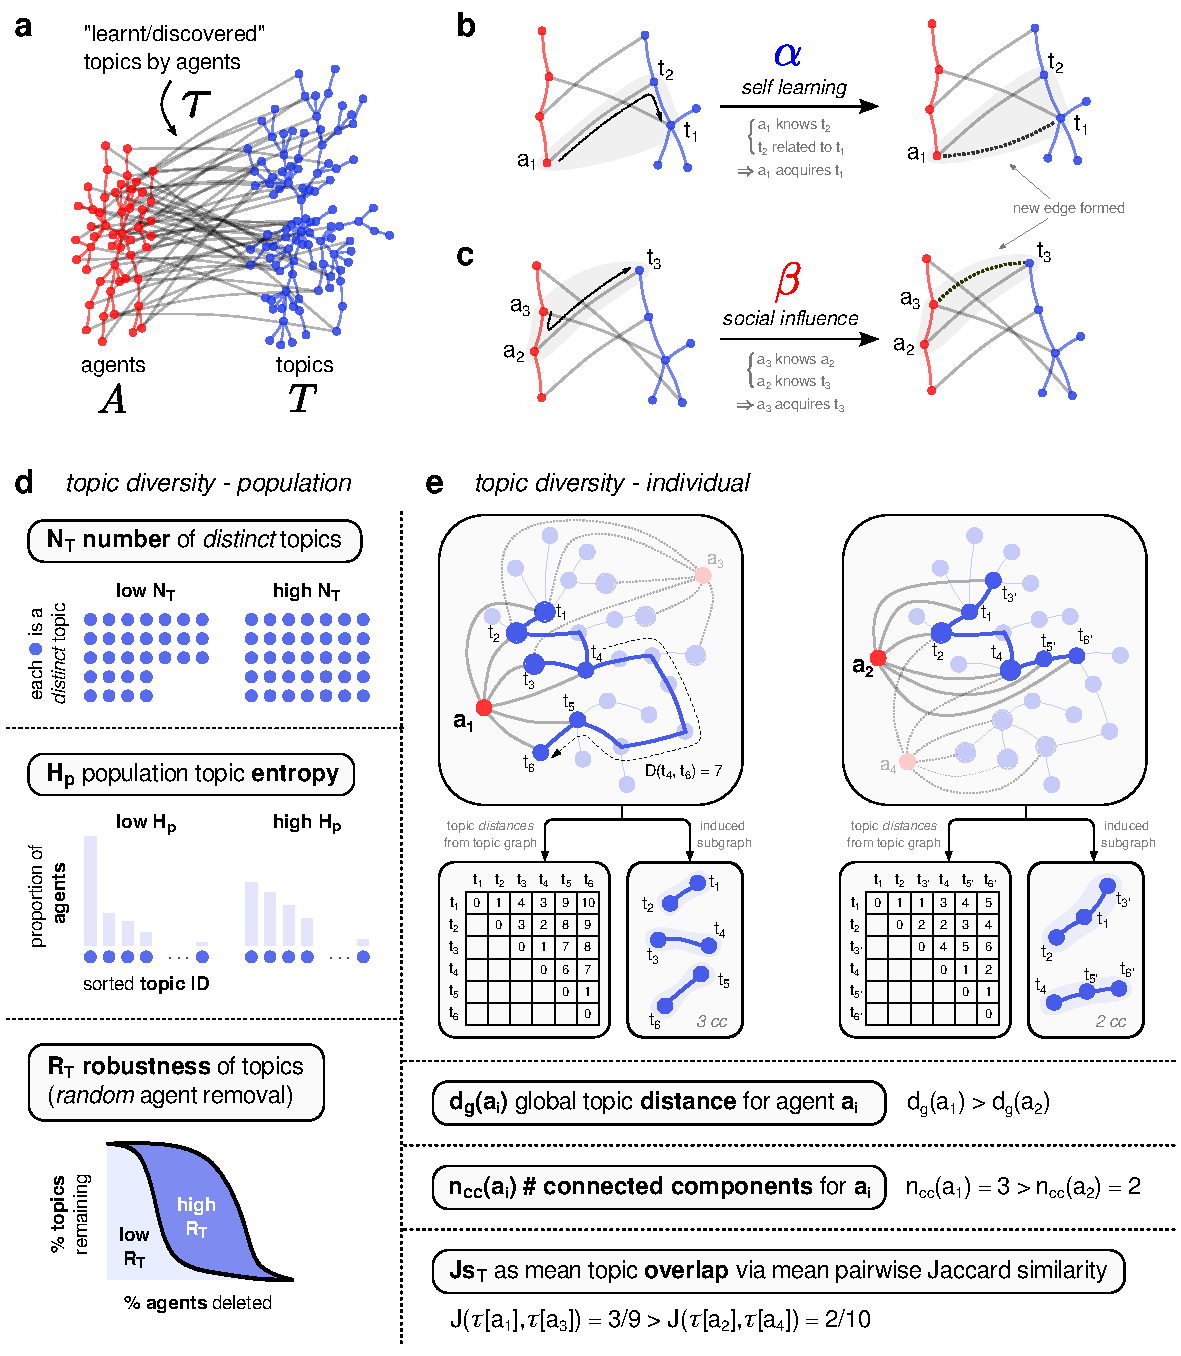
\includegraphics[width=\textwidth]{Fig1.pdf}
    \caption{
    \textit{Description of the topic update/discovery process in the model and the different knowledge diversity metrics}.
    (\textbf{a}) Illustration of the intralayer agent graph (\textit{red}) and topic graph (\textit{blue}) with the interlayer edges (\textit{gray}) representing the knowledge set of the agents.
    \textit{Gray} cartoon triangles in (\textbf{b}) and (\textbf{c}) illustrate the update process either through learning/discovery by related topics (self-learning) or learning/discovery through friends (social influence).
    (\textbf{d}) Illustrations of different diversity metrics at the population level (each blue circle is a topic).
    (\textbf{e}) Illustrations of topic diversity metrics at the individual and local level (see \textbf{Sect. \ref{sec:method-diversity}} for detailed descriptions).
    }
    \label{fig:1}
\end{figure}

\subsubsection*{General description}

All models considered here are binary undirected graphs. There are $n_a = 200$ agents and $n_t = 1000$ topics. Denote $A$ and $T$ as the symmetric binary adjacency matrices of the agent graph $G_a$ and topic graph $G_t$ respectively (\textbf{Fig. \ref{fig:1}}a). The bipartite incidence matrix $\tau$ of size $n_t \times n_a$ represents the topics that the agents know about. It is assumed throughout that the intralayer edges are static while the interlayer edges could be \textit{acquired} through the update process. And once an interlayer edge is acquired, it is assumed to be persistent. At the initial stage, each agent is assigned at most $\tau_0 = 5$ topics with certain probabilities based on the models of the intralayer models (see below). There is also an upper limit topic capacity $\tau_{\mathrm{max}} = 50$ per agent, and the update process is only simulated until $1.2 \tau_{\mathrm{max}} = 60$ time steps. For each parameter set ($\alpha$, intralayer models, interlayer initialization), I ran 5 simulations each.

\vspace{-1em}
\subsubsection*{Update of interlayer edges}

At each time step, at most one new topic is learnt per agent. The agent could acquire a new topic edge either through the self-learning strategy with $\alpha$ probability, by learning about the related topics of things an agent already knows about (\textbf{Fig. \ref{fig:1}}b). On the other hand, with probability $\beta$, an agent could acquire a new topic edge by traversing its neighbors in the agent graph then to the topic graph (\textbf{Fig. \ref{fig:1}}c). One way to implement this is below.

Define $\psi(X)$ as a column L1 normalization operation on a matrix $X$, i.e. each column vector $\vec{x}_i$ of the matrix is normalized to $\vec{x}_i/||\vec{x}_i||_1$. Define the shorthand notation for the Heaviside function as $[x]_{\star} = 1$ if $x > 0$, and $0$ otherwise. At each time step, the probability matrix $P$ (of same size as $\tau$) with its column vector $\vec{p}_i$ defining the probability agent $a_i$ choosing a new topic. A way to define this probability is:

\vspace{-1em}
\begin{eqnarray}
    P &=&
    \alpha \psi\left(\left[\left[T\tau\right]_{\star} - \tau \right]_{\star}\right) +
    \beta \psi\left(\left[\left[\tau A\right]_{\star} - \tau \right]_{\star}\right)
    \label{eq:1}
    \\
    \tau(t+1) &\leftarrow& \tau(t) + \texttt{sample}(P)
    \label{eq:2}
\end{eqnarray}

The multiplication steps perform the traversal through neighbors across the intralayer networks. The binarization and subtraction with the current $\tau$ simplifies the implementation, to only learn new topics and to balance not being stuck around too popular topics. Additionally, for simplicity here I consider $\beta = 1 - \alpha$ so the process is only defined by $\alpha$. Many other probabilities are ignored as well, for example serendipity (wandering or random discovery of new topics) and forgetting (removal or decrease of strength of interlayer edges).

\vspace{-1em}
\subsubsection*{Intralayer random models}

For simplicity, the model types and model hyper-parameters (except only for the number of nodes) are similar the same for agent and topic graphs for each simulation.

\textit{Nonblock models}: The first approach is non-block networks. In the main text, I analyze the model scale-free network (SF), constructed by the linear from preferential attachment models (\texttt{PA}) \cite{Barabasi1999-dw} (see \textbf{Fig. \ref{fig:2}}). Additionally, I also analyze nonlinear \texttt{PA} models, Erdős–Rényi (\texttt{ER}) networks \cite{Erdos1959-dj} with different connectivity probability, as well as small-world networks generated with the Watts–Strogatz (\texttt{WS}) models \cite{Watts1998-vh} (see \textbf{Fig. \ref{supp:1}}a).

\textit{Block models}: Since in real-world networks, there are usually communities (researchers or papers within the same field), I also use the stochastic block models (\texttt{SBM}) \cite{Faust1992-xo} to emulate this with $k_a = k_t = 10$ groups for both agent and topic networks. A way to manipulate these models is to change the probability of connection within groups ($p_{\mathrm{within}}$) or between groups ($p_{\mathrm{between}}$). For simplicity, I kept the former the same while varying the latter (see \textbf{Fig. \ref{fig:3}}).

\vspace{-1em}
\subsubsection*{Interlayer initialization}

Generally at the initialization stage, the probability of connection between a given agent and topic could be the same across topics. However, it is possible that other initialization strategies might bias the results in one way or another. Hence, I introduce two different interlayer initialization strategies, one for \textit{nonblock} intralayer models and one for \textit{block} models. Whenever an initialization method is not mentioned, it is assumed to be the uniform random strategy.

For \textit{nonblock} intralayer models, the probability of connecting to a certain topic could be dependent on its degree in $G_t$. A way to do this is to perform the $\texttt{softmax}\left(\{d_i\}; \beta_{\sigma}\right)$ on the degrees, basically transforming the degree sequence $\{d_i\}$ to a probability distribution. With $\beta_{\sigma} < 0$ ($\texttt{SOFTMAX}_1$), low degrees are favored; $\beta_{\sigma} = 0$ is equivalent to random initialization ($\texttt{SOFTMAX}_2$), while $\beta_{\sigma} > 0$  ($\texttt{SOFTMAX}_3$) favors high degree topics (\textbf{Fig. \ref{supp:2}}a)

For \textit{block} intralayer models, group correspondence could be used as a strategy for initialization as the number of groups are the same for both graphs. This could be parameterized by $p_{sg}$ (\textbf{Fig. \ref{fig:3}}) as the probability that agents and topics of the same group ID are connected. The chance $p_{sg} = \frac{1}{k_t} = 0.1$ would be equivalent to random initialization.

\subsection{Diversity metric} \label{sec:method-diversity}

The concept of knowledge diversity
These diversity metrics are illustrated in \textbf{Fig. \ref{fig:1}}d,e.

\vspace{-1em}
\subsubsection*{Population}

Three population indices are defined, taken from ecological perspective \cite{Tuomisto2010-pr}. First, $N_T$ is the number of distinct topics discovered when taking into account all agents' learnt topics (higher would mean more diverse). Second $H_p$ is the topic population entropy -- the Shannon entropy from the discrete probability distribution of all the topics in the population (higher would mean more diverse). Lastly, taken inspiration from ecological network stability analysis \cite{Memmott2004-os}, robustness can be calculated by cumulatively removing random agents and observing the remaining \% of distinct topics. The area under this curve is the robustness $R_T$ (higher would mean a lot of agents are needed to be removed to remove a large proportion of topics).

\vspace{-1em}
\subsubsection*{Individual}

Three individual indices are calculated and the averaged computations across nodes (or pairs) of the agent graph are reported. First, $d_g$ is the mean distance of the topics in each agent's learnt topics. In other words, if we define $D(t_i,t_j;G_t)$ as the shortest path distance in $G_t$ between $t_i$ and $t_j$, and an agent $a_k$'s topic set as $\tau[a_k] = \left\{t_h | \tau[t_h,a_k] = 1 \right\}$ then $d_g(a_k) = \left\langle D(t_i,t_j;G_t)\right\rangle_{t_i, t_j \in \tau[a_k]}$. Higher on average would suggest that the agents know more out of their comfort zone and tend more towards generalists. Another metric is the number connected component $n_{cc}(a_k)$ of the induced subgraph $G_t(\tau[a_k])$ -- higher would mean there are many ``islands'' of topics that the agent knows about, leaning toward generalist trend. Lastly, the mean pairwise Jaccard similarity $Js_T$ between agents' topic sets are calculated, lower would mean higher local diversity on average.

\vspace{-1em}
\subsubsection*{Group}

Additionally, when groups are defined in the block intralayer models, one could also calculate the entropy of the topic group distribution, in both the population sense $H_{gp}$ and individual sense $H_{gi}$. More specifically, $H_{gp}$ is the entropy of the 10 topic groups when taking into account the group identities of all topics learnt by all agents. On the other hand, $H_{gi}$ is the average entropy of each agent's own topic entropy. These two quantities are different, e.g. there could be cases where $H_{gp}$ is maximized (all groups uniformly distributed) but $H_{gi}$ could be 0 (each agent only learns about the topics within the same group).

\subsection{Code availability}

The source code is at \url{https://github.com/tuanpham96/topic-diversity}. The simulations were run in parallel on Azure VM.

\section{Results}

\begin{figure}[!ht]
    \centering
    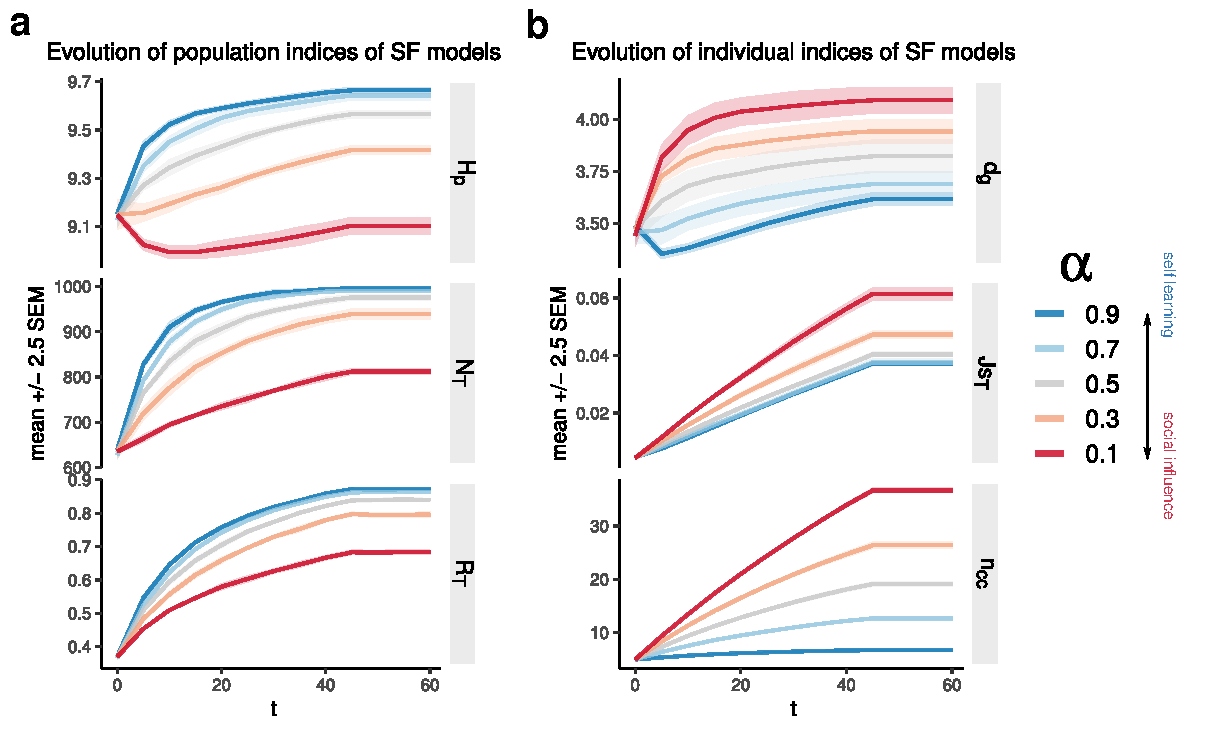
\includegraphics[width=\textwidth]{Fig2.pdf}
    \caption{
    \textit{Changes of population topic diversity indices} (\textbf{a}) \textit{and of individual diversity indices} (\textbf{b}) \textit{of the scale-free (SF) intralayer models} \textit{due to} $\alpha$. $H_p$: topic population entropy; $N_T$: number of distinct topics; $R_T$: robustness due to \textit{random} removal of agents; $d_g$: mean distance of the subset of topics that agents know; $Js_T$: Jaccard similarity of topic set between agents; $n_{cc}$: number of connected components of induced subgraphs based on each agent's learnt topics. See \textbf{Sect. \ref{sec:method-diversity}} and \textbf{Fig. \ref{fig:1}}d,e for more details. Each line represents the mean changes of 5 realizations, analyzed every 5 steps.
    }
    \label{fig:2}
\end{figure}

\subsection{\textit{Nonblock} intralayer models} \label{results-nonblock}

The changes of the different diversity metrics for the scale-free networks are shown in \textbf{Fig. \ref{fig:2}} as an example to illustrate the tradeoff effect of the self-learning versus social influence probability on the population and individual diversity.

Generally, topic population diversity increases with self-learning probability $\alpha$ in terms of the topic entropy $H_g$ and number of topics $N_T$. Through learning/discovery through time, low $\alpha$ could still achieve better population diversity. However, it does not seem likely for the worst case considered here, where entropy does not even increase considerably pass its initial value. The initial decrease of $H_g$ when $\alpha = 0.1$ is because the agents start learning from each other, hence temporarily creating bias towards some topics, leading to decrease of entropy. It must be noted here that the entropies are already high initially due to initialization. However, taking the trends of both $N_T$ and $H_g$ into account, it is reasonable to say that higher $\alpha$ improves topic population diversity. Additionally, higher $\alpha$ leads to more robust retainment of the topics under random agent removal (i.e. higher $R_T$).

On the other hand, topic individual diversity usually decreases based on the chosen metrics. Increased $\alpha$ leads to decreased mean learnt topics distance $d_g$ and number of components $n_{cc}$ in the induced subgraphs. Intuitively, higher social influence  -- lower $\alpha$ -- would allow the agents to access topics out of their comfort zone easier, hence their own subgraph of topics tend to be more generalist, whereas higher $\alpha$ leads to more specialization. Lastly, at the local level $Js_T$, lower $\alpha$ leads to more similarity between neighbors, hence lower local diversity. Although not analyzed, this hints at how social influence could create modularity in the learnt topic graph $\tau$.

These trends are quite consistent across different considerations of non-block models (\textbf{Fig. \ref{supp:1}}). Increasing in $\alpha$ leads to higher topic population diversity ($N_T, H_p$), robustness ($R_T$) and local diversity ($Js_T$). On the other hand, such increases tend to result in loss of topic individual diversity ($d_g$, $n_{cc}$). When taking into account degree-dependent initialization strategies (\textbf{Fig. \ref{supp:2}}), favoring more obscure topics leads to the same trend as random initialization. However, initially favoring more popular topics actually would be detrimental generally across different population, local and individual diversity indices, especially for those networks generated by preferential attachments (\texttt{PA}) models, possibly because learning more easily gets stuck in the topics connected to the popular ones (last row in \textbf{Fig. \ref{supp:2}}b).


In summary, in non-block intralayer models, higher self-learning $\alpha$ leads to higher topic diversity in a local and population context, but whereas higher social influence encourages higher individual topic diversity. Initialization favoring more popular topics seems to have a negative effect on these different metrics.

\begin{figure}[!ht]
    \centering
    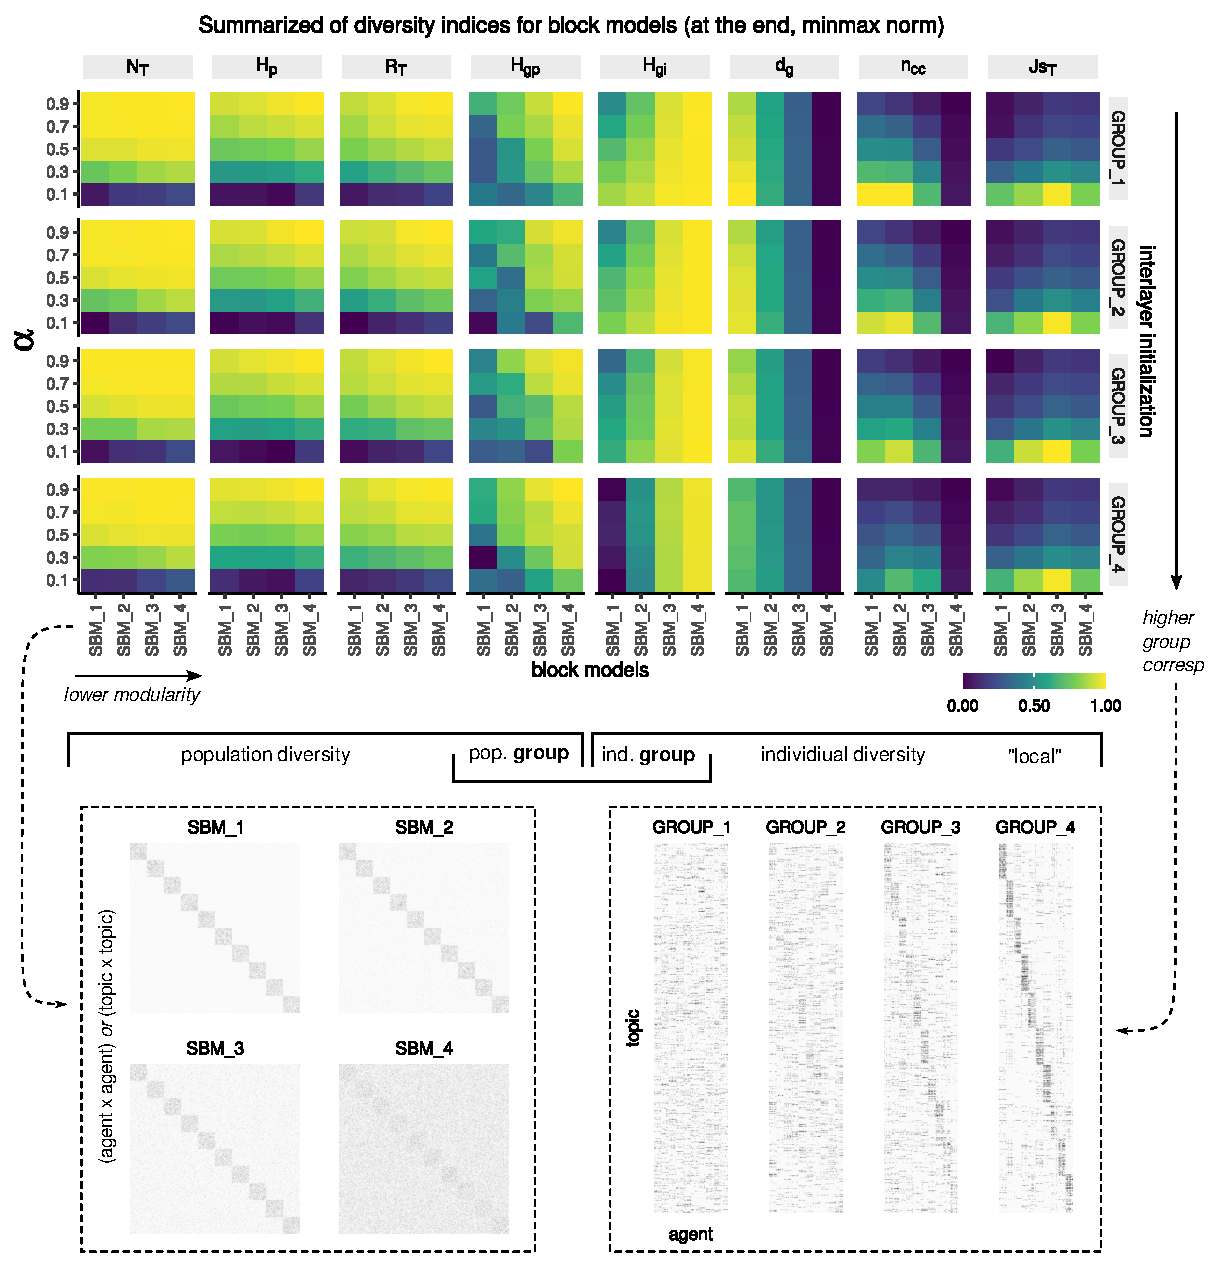
\includegraphics[width=\textwidth]{Fig3.pdf}
    \caption{
    \textit{Summary  of  population  and  individual  diversity  indices  due  to $\alpha$,  across  different  block  models}. Within each heatmap, x-axis shows decreasing modularity of intralayer model (via increasing inter-modular connectivity), y-axis is $\alpha$. The color represents values at the end of the simulations, and min-max normalized within each metric. From left to right are different diversity metrics. From top to bottom are different group correspondence initialization strategies.
    }
    \label{fig:3}
\end{figure}


\subsection{\textit{Block} intralayer models and topic group diversity}
\label{results-block}

As real-world networks usually contain communities within them, I use the stochastic block intralayer models (\texttt{SBM}) to observe how diversity indices change due to $\alpha$ and network modularity. Generally, the trends for population diversity and robustness during the simulation are similar from previously discussed (\textbf{Fig. \ref{supp:3}}a). The trends as a function of model modularity do not seem to differ much either. Looking at the group population entropy $H_{gp}$ (\textbf{Fig. \ref{supp:3}}b, bottom), only when the networks are less modular do such values show a difference, albeit very small.

In the individual perspective (\textbf{Fig. \ref{supp:3}}c), group modularity actually helps with diversity indices $d_g$ and $n_{cc}$, possibly because there are fewer long-range links. The trends for local diversity are roughly similar and not affected much by group modularity. Additionally, instead of only looking at topic group diversity in the population sense, one could also inspect it in the individual perspective. On average (\textbf{Fig. \ref{supp:3}}b, top), for more modular intralayer networks, social influence benefits topic group diversity in the agents, because the agents would have higher chance to learn out of their own comfort zone, especially if their initial topics belong to the same groups. With decreasing group modularity, these differences between $\alpha$ do not seem to matter any more.

Inspecting the end values of these different metrics in \textbf{Fig. \ref{fig:3}} taken into account group-correspondence initialization strategies reveal these effects more clearly.

More specifically, higher $\alpha$ and lower intralayer modularity generally leads to higher population topic diversity and robustness ($N_T, H_p, R_T$), whereas group correspondence initialization does not seem to have pronounced effects. Group modularity benefits the individual diversity ($d_g, n_{cc}$) but high initial group-correspondence would counter such effects, as learning gets stuck within communities. At the local level, group-correspondence does not seem to affect $Js_T$ visibly. However, generally higher $\alpha$ and higher model modularity tends to decrease topic similarity, hence increasing local diversity.

When we start to consider group entropies, generally low group modularity increases both topic group population ($H_{gp}$) and individual ($H_{gi}$) diversity. High initial correspondence though seems to benefit group population diversity (although such benefits may be small, see \textbf{Fig. \ref{supp:3}}b), it seems to decreases group individual diversity.

In summary, with consideration of intralayer block models, higher $\alpha$ still benefits more for population diversity and robustness, but not so much with group population diversity. in the presence of high social influence, high network modularity may hurt population diversity, regardless of initial group-correspondence. On the other hand, lower $\alpha$ is generally more beneficial for individual indices like discussed with SF models, including group individual diversity, but either low network modularity or high group correspondence would tend to be harmful for these metrics. At the local level, higher $\alpha$ and high network modularity tends to be more beneficial for decreasing similarity between agents.

\section{Discussion}

In conclusion, with this simple toy model of topic discovery and a simple update rule depending on the probability of traversing through neighbors of bipartite networks, some interesting results are obtained. First of all, increasing $\alpha$ (self-learning, traversing through interlayer edges first) leads to higher topic population diversity and robustness in various random models for the intralayer networks, including blocks and non-block models. However, such increase has drawbacks when looking at topic individual diversity, as it reduces the chance for the agent nodes to acquire interlayer edges from topics that are usually out of their comfort zone. Social influence, traversing through intralayer edges first ($\beta$ route) would better benefit individual diversity.

When groups are considered in the intralayer networks, group modularity may hurt the population diversity (though some only by a little) and more apparently for group individual entropy, though interestingly more beneficial for individual indices through the lense of graph distances and components. Although initial group correspondence does not have much effects on the population diversity, it has a dramatic drawback at the individual level (both entropy and graph metrics).

% \vspace{-1em}
% \subsubsection*{Limitations and considerations}

Though there are interesting results in a theoretical sense as a toy model, there are quite many limitations of the current model. Future studies should relax the assumptions made here and test out different versions of the models, e.g. different ratios between intralayer network sizes, inclusion of directed weighted edges (strengths could imply confidence in knowledge in $\tau$), non-persistent interlayer edges, different update probabilities (serendipity, forgetting, strengthening, ...), the cost of learning new subjects, delays in acquiring new knowledge, different versions of the update equation and, more importantly, the dynamic nature of the intralayer networks (e.g. \cite{Sun2020-qj}) and the decreased disruptiveness in new knowledge discovery \cite{Park2021-jb}. Furthermore, future endeavours should take into account performing the update process in real networks, which could be constructed using, as an example, the citation networks (agents as authors, papers as topics, groups as fields or subfields) or social networks \cite{Weng2015-zt}. Additionally, further analyses include examination of the modularity changes in the bipartite $\tau$ \cite{Dankulov2015-uv} or in the projected graphs (for example, low $\alpha$ might start to create communities as evidenced by high Jaccard similarity in these simulations), the distribution of specialists and generalists, different local diversity definitions (e.g. topic entropy as a function of distance from a given agent) and persistent homology analyses (since the interlayer edges are defined as persistent here).

\section{Acknowledgement}

I would like to thank Dr. Mercedes Pascual and Dr. Sergio A. Alcala Corona, my friends Sam Nguyen and Poojya Ravishankar for their discussion and feedbacks of the model and interpretations.

\bibliographystyle{splncs03}
\bibliography{library}

\vspace{-1em}

\section*{Supplementary figures}

\setcounter{figure}{0}
\renewcommand{\thefigure}{S\arabic{figure}}

\begin{figure}[!ht]
    \centering
    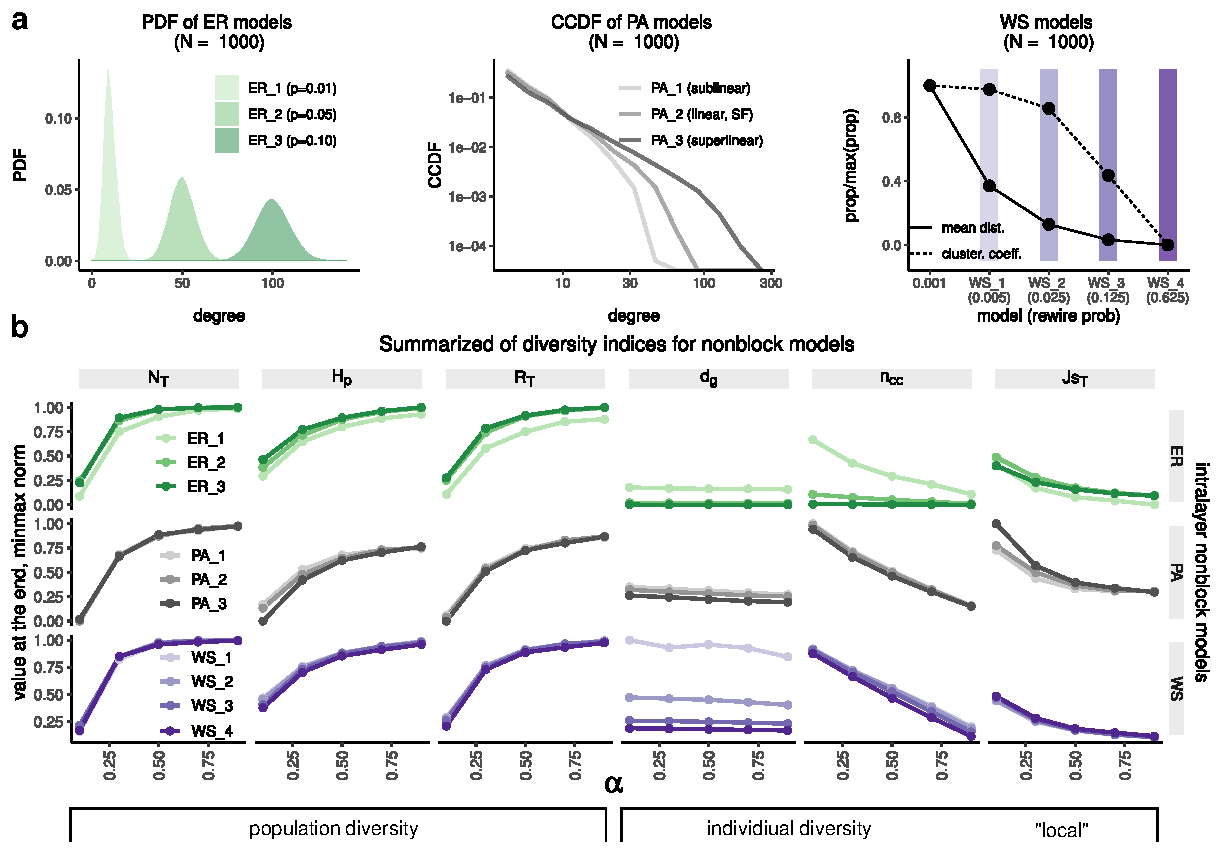
\includegraphics[width=0.9\textwidth]{FigS1.pdf}
    \caption{
    \textit{Variations of nonblock intralayer models}.
    (\textbf{a}) Set up of nonblock models. \texttt{PA}: preferential attachment, \texttt{ER}: Erdős–Rényi, \texttt{WS}: Watts–Strogatz (\textbf{Sect. \ref{sec:method-model}})
    (\textbf{b}) Changes of diversity indices for these models as a function $\alpha$ (\textbf{Sect. \ref{sec:method-diversity}})
    }
    \label{supp:1}
\end{figure}

\begin{figure}[!ht]
    \centering
    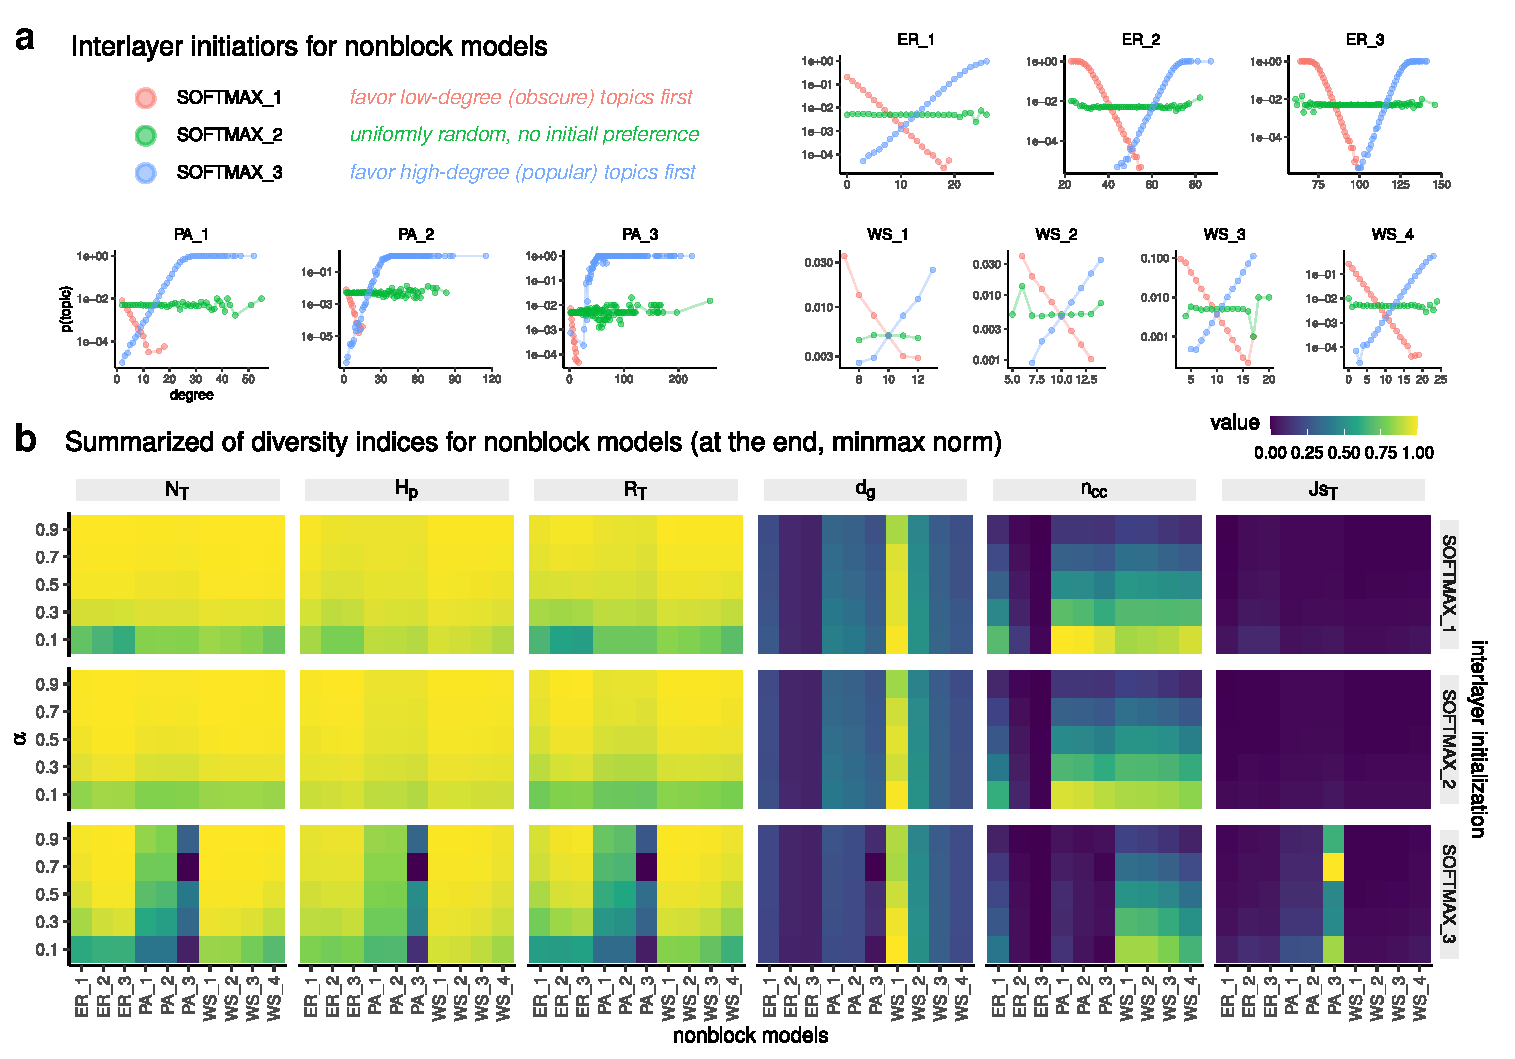
\includegraphics[width=0.95\textwidth]{FigS2.pdf}
    \caption{
    \textit{Different initialization strategies for nonblock models} (\textbf{a}) \textit{based on the topic intralayer degrees and }(\textbf{b}) \textit{effects on population and individual diversity indices as a function of $\alpha$}. See \textbf{Fig. \ref{supp:1}}a for names and illustrations of the different models.
    }
    \label{supp:2}
\end{figure}

\begin{figure}[!ht]
    \centering
    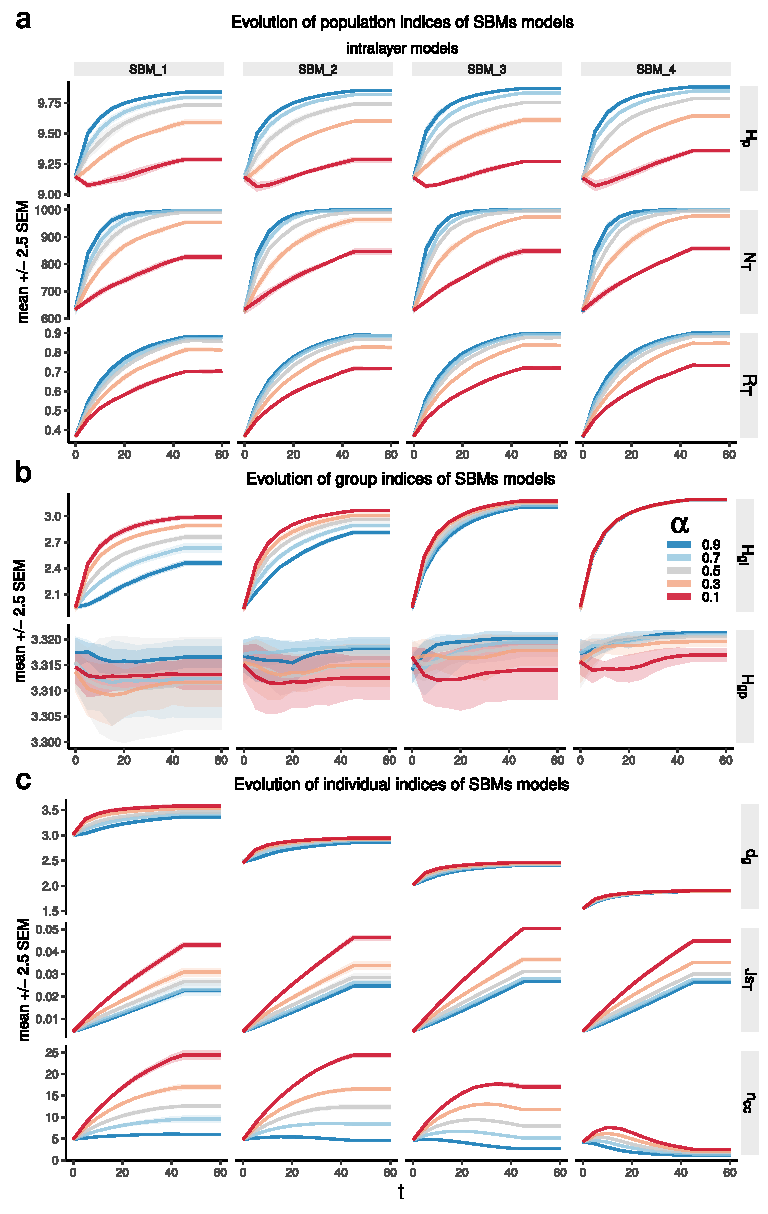
\includegraphics[width=0.85\textwidth]{FigS3.pdf}
    \caption{
    \textit{Changes of population diversity indices} (\textbf{a})\textit{, group diversity indices} (\textbf{b}) \textit{and individual diversity indices} (\textbf{c}) \textit{for the stochastic block intralayer models} \textit{due to} $\alpha$.
    }
    \label{supp:3}
\end{figure}

\end{document}
